%!TEX root = ./thesis.tex

\chapter{Hardware implementation}
\label{cha:hard}

A hardware implementation consist in a set of file written in \gls{hdl} with constraints associated to these files. First, I describe the hardware implementation of operations on posit numbers, namely addition and multiplication which are the basic building blocks of \glspl{spn}. Then I explain how \glspl{spn} hardware files are generated from a trained \gls{spn} file. Finally, I describe the implementation of the \gls{spn} inside the \gls{fpga} with the complete control scheme. The design is intended to work on a Zed Board.

% ==============================================================================
\section{Hardware operators}
% ==============================================================================

In this section, I describe how posit operations are performed in hardware. The general schematic is described in Figure \ref{fig:posit_op}. The floating point operation mentioned here represents the operation described in Algorithm \ref{alg:float_add} and \ref{alg:float_mult}. For a posit operation, the size of each field must be properly computed and is different from a classical floating point operation.

\begin{figure}[!ht]
\begin{mdframed}
	\centering
	\includestandalone[width=\linewidth]{../Images/operator}
	\caption{Illustration for posit operations. With a posit number of $N$ bits and $es$ exponent bits, the size of the significand is equal to ($N-2-es+1$) and the size of the exponent is equal to ($\log_2(N)+es+1$)}
	\label{fig:posit_op}
\end{mdframed}
\end{figure}

% ------------------------------------------------------------------------------
\subsection{Encoder and Decoder}
% ------------------------------------------------------------------------------
As posit representation use variable size fields, an encoder and decoder are required to extract useful information from a raw binary sequence. The useful information consists in a significand and an exponent (the exponent mentionned here corresponds to the real exponent of \ref{fig:posit_shema} which combines the exponent fields and the regime).

The decoder schematized in Figure \ref{fig:dec_mod} must extract the different quantities of a posit number to transform it into a useful format for computations. First it must retrieve the value of the real exponent. To do so, a leading zero counter can extract the value of the regime. Once the regime is found, the position of the exponent is known and can also be extracted. This extraction is done using shifting operators. These operators have the advantage to ignore the fact that the exponent bits may not be encoded due to the regime size. Then it must extract the value of the significand. This is similar to the extraction of the exponent.

The encoder schematized in Figure \ref{fig:enc_mod} is conceptually the opposite of the decoder. It takes three inputs: A regime value (in 2's complement), an exponent value (usingned int) and a significand (unsigned int). First it extract the regime size as well as a regime writen in unary notation. Then it uses the regime size to shift the exponent and significand to place them at the correct place in the posit number.

\begin{figure}[!ht]
\begin{mdframed}
	\centering
	\subfloat[Decoder]{\includestandalone[width=\linewidth]{../Images/decoder_module_2}\label{fig:dec_mod}}

	\subfloat[Encoder]{\includestandalone[width=\linewidth]{../Images/encoder_module_2}\label{fig:enc_mod}}
	\caption{Logical blocks for the encoder and decoder using shifts. Outputs of the decoder and input of the encoders are the regime (in 2's complement), the exponent (unsigned integer) and the significand (usigned integer). In order to get the value of the real exponent mentionned in Figure \ref{fig:posit_shema}, the regime and the exponent field have to be concatenated. The leading digit count compute the value of the regime and the size of the regime. The regime writer build a regime in unary notation and output the regime size. N and es are constant and represent the number of bits and the exponent size of the posit number. rs is the regime size and is dynamically computed.}
\end{mdframed}
\end{figure}



% \begin{figure}[!ht]
% \begin{mdframed}
% 	\subfloat[Decoder]{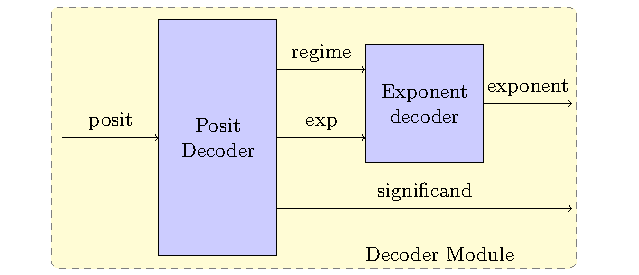
\includegraphics[width=0.49\linewidth]{../Images/decoder_module} \label{fig:dec_mod}}
% 	\subfloat[Encoder]{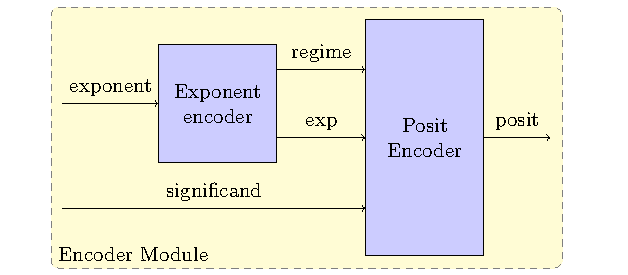
\includegraphics[width=0.49\linewidth]{../Images/encoder_module} \label{fig:enc_mod}}
% 	\caption{Schematic of encoder and decoder modules}
% 	\label{fig:enc_dec_mod}
% \end{mdframed}
% \end{figure}

% ------------------------------------------------------------------------------
\subsection{Adder and multiplier}
% ------------------------------------------------------------------------------
Once posit numbers are decoded into a single exponent and a significand, performing an addition or a multiplication is the same as the application of an addition or a multiplication in the context of floating point numbers as shown in Figure \ref{fig:posit_op}.

From \ref{fig:posit_op}, it is easy to conceive that a posit operation consume more hardware resources than a floating point operation since posit operations requires two encoders and one encoder. Note that even the floating point operation performed in the posit operator is bigger than a standard posit operation because the exponent and the significant must be big enough to represents the entire range of posit. The significand size is then of $(N-2-es+1)$, and the exponent size of $(\log_2(N)+es+1)$.

As a reminder, the benefit of using posit is that the range of representable number is increased and that a large set of number can be encoded using more fraction bits than floating point representation.


% ==============================================================================
\section{Sum product networks}
% ==============================================================================

\Glspl{spn} are built using only adders and multipliers. The challenge of this section is that there exists many different architecture of sum product networks, and that there can be thousands of nodes in a single \gls{spn}. Therefore, the process of generating a \gls{spn} in \gls{hdl} from a trained one is automatized.

As inputs, it takes a file containing a trained \gls{spn} in the form of a \gls{psdd}. It outputs a HDL file representing the \gls{spn} with all the weights in posit representation. The inputs of the \gls{spn} are binary units because there are only zeros or ones. The first layer of the \gls{spn} consist in converting these inputs into posit numbers.

% ------------------------------------------------------------------------------
\subsection{Pipelining}
% ------------------------------------------------------------------------------
A \gls{spn} can be built using only basic building block such as adder and multiplier, but it would be very slow since the depth of the \gls{spn} can be high. Every time a new input would be sent, the output would be available after the longest datapath in the network is crossed. Furthermore, it would induce a high consumption of switching power. Therefore it is a good idea to pipeline the path from input to output in order to increase the maximum frequency and reduce the power consumption.

One can not simply add a register at every input or output of every nodes since some values can skip multiple layers at once. In order to pipeline properly the entire \gls{spn}, the depth of each node must be computed and an appropriate number of register must be set on each path. As shown in Figure \ref{fig:pip}, some paths may cross different pipeline stage and require multiple registers.

In addition to this, a valid signal flow through the pipeline. This signal is useful to synchronize the output of the \gls{spn} with the rest of the architecture. Whenever a new input is given to the \gls{spn}, valid is set to one, and flow up to the output. And whenever a valid equals to one is read at the output of the \gls{spn}, it means that the output was generated from a valid input.

\begin{figure}[!ht]
\begin{mdframed}
	\centering
	\includestandalone{../Images/pipeline}
	\caption{Pipelining of SPN. A new register is added every time a path cut a depth level. Valid signals flow through the pipeline to assert that values in this layers are generated from a valid set of inputs. Here valid means that it is a set of inputs sent by the user, it may not be valid in the definition of a \gls{spn}.}
	\label{fig:pip}
\end{mdframed}
\end{figure}


% ==============================================================================
\section{Global system}
% ==============================================================================

The global system shown in Figure \ref{fig:glob_workflow} show the three main part of the structure: The \gls{fpga}, the control unit and the memory.

\begin{figure}[!ht]
\begin{mdframed}
	\centering
	\includestandalone[width=\linewidth]{../Images/big_picture}
	\caption{Architecture of Zed Board. The \gls{fpga} contains the \gls{spn}, an input module to parallelize the inputs and a \gls{fifo} to synchronize the outputs. The memory contains the software to be exectued by the \gls{cpu} and a list of inputs to be sent to the \gls{fpga}. The \gls{cpu} controls the entire structure through \gls{axi} communication.}
	\label{fig:glob_workflow}
\end{mdframed}
\end{figure}

% ------------------------------------------------------------------------------
\subsection{FPGA}
% ------------------------------------------------------------------------------

Once the \gls{spn} is built, it must be integrated into a structure to be able to properly push inputs and get outputs. Two major problems are faced. Firstly, the number of inputs of a \gls{spn} may be high and we are limited to a 32 bits per clock cycle using the AXI interface. Secondly, the \gls{spn} works at a lower frequency than the rest of the hardware, so some clock domain crossing would be necessary to integrate the \gls{spn} inside a system.

In order to solve the problems of the number of inputs, a module whose function is to parallelize the inputs must be added in the \gls{fpga}. It is called here \textit{input module}. The input width of the input module is limited to 32 bits (AXI interface) and works at a high frequency. The output width of the input module is the number of different literals of the \gls{spn}.

The different frequencies in the global systems are shown by the colors in Figure \ref{fig:glob_workflow}. In order to maximize throughput and perform a clock domain crossing, a \gls{fifo} is placed at the output of the \gls{spn}. The input of this \gls{fifo} works at a low frequency (\gls{spn} frequency) and the output works at a high frequency (AXI frequency).

The \gls{fpga} is size limited. Not all \gls{spn} will fit inside it. The key limiting factors are the number of slice \glspl{lut} and the number of \glspl{dsp}. A Zed Board possesses 53200 slice \glspl{lut} and 220 \glspl{dsp}.

\todo{In answer to Nimish's comment: The biggest size of the \gls{spn} that fits on the Zed Board is mentioned in the results. Should it be also written here ?}

% ------------------------------------------------------------------------------
\subsection{Memory}
% ------------------------------------------------------------------------------
The memory initially contains the software to be executed as well as the set of inputs for which we want to compute the probability.

% ------------------------------------------------------------------------------
\subsection{Control unit}
% ------------------------------------------------------------------------------
The control unit execute the software. It should send data to the \gls{fpga} and receive the output from the \gls{spn}. The maximum frequency of the \gls{fpga} is known by design. Therefore we can just push the data at the best frequency that will not break the \gls{spn} and get the data. Once the data is received, it is sent over stdout which can be accessible through \gls{jtag} to get the data out of the Zed Board.




